% Presentation defs:
\documentclass[mathserif,10pt]{beamer}
\usepackage{amsmath}
\DeclareMathOperator{\Hessian}{Hess}
\DeclareMathOperator{\Tr}{Tr}
% Handout defs:
%\documentclass[mathserif,10pt,handout]{beamer}
%\usepackage{pgfpages}
%\pgfpagesuselayout{2 on 1}[a4paper,border shrink=5mm]
%\setbeamertemplate{footline}{\scriptsize{\vspace*{-0.3cm}\hspace*{0.95\textwidth}\insertframenumber}}
% End of handout defs:


%
%%**********************************************************
%%********* Auxiliary packages *****************************
%%**********************************************************
%-----------------------------------------------------------
%---- Language: Hyphenation etc. ---------------------------
%\usepackage{german}%die alte Rechtschreibung
%\usepackage{ngerman}%die neue Rechtschreibung
%\usepackage[ngerman]{babel}%babel+neue Rechtschreibung
%
%-----------------------------------------------------------
%---- Zeichenkodierung bei Quellcode: ----------------------
\usepackage[utf8]{inputenc}%deutsche Zeichen: Eingabe mit Umlauten
%
%-----------------------------------------------------------
%---- Schriftkodierung bei Ausgabe: ------------------------
%\usepackage[T1]{fontenc}%Umlaute, Ligaturen, besserer Zeilenumbruch
%\usepackage{t1enc}%Gleiche Wirkung wie die obere Zeile? Oder gar besser?
%
%-----------------------------------------------------------
%---- Math-Pakete: -----------------------------------------
%\usepackage{amstex}%ist veraltet
\usepackage{amsmath}
\usepackage{amsmath}
\usepackage[mathscr]{euscript}%so liefern '\mathcal' und '\mathscr' verschiedene Zeichen
\usepackage{amssymb}
%\usepackage{amsthm}% Theoremumgebungen u.s.w. -- kollidiert mit beamer/hyperref
%\usepackage{latexsym}%was war das nochmal?
\usepackage{exscale}%Summen-und Integralzeichen in richtiger Größe
%
%-----------------------------------------------------------
%---- Grafik-Pakete: ---------------------------------------
\usepackage{graphicx}%graphicx: extended graphics-Package, ist moderner
%\DeclareGraphicsExtensions{pdf,jpeg,gif}%Priority of graphic types, if needed
\usepackage{psfrag}
\usepackage{xspace} 
\usepackage{enumerate}
\usepackage{pgf}
\usepackage{xcolor}%extended color-Package, denke ich
\usepackage{latexsym}
\usepackage{subfigure}
\usepackage{hyperref}

%***********************************************************
%***** Beamer-layout für slides und handout ****************
%***********************************************************

%
%***********************************************************
%***** Beamer-Theme-Einstellungen **************************
%***********************************************************
\mode<beamer>{ %gilt nur in Beamerversion
\usetheme{Winterthur}
}
%\xdefinecolor{brickred1}{RGB}{229,79,57} % cmyk{0,66,75,10}
% \xdefinecolor{brickred2}{RGB}{204,70,51} % cmyk{0,66,75,20}
\xdefinecolor{MyNewDelftBlue}{RGB}{81,126,218}
\xdefinecolor{MyRed}{RGB}{255, 48, 0}
\xdefinecolor{MyOldPaper}{RGB}{249, 242, 221}
%
%\usecolortheme[RGB={0,0,220}]{structure}
% Winterthur bright:
%\usecolortheme[RGB={41,91,229}]{structure}
% Winterthur middle:
%\usecolortheme[RGB={61,108,224}]{structure}
% Winterthur soft: (++ die Struktur ist fröhlich, tritt aber optisch zurück) 
\usecolortheme[RGB={81,126,218}]{structure}
% Cool dark blue? (+ die Struktur ist sehr solide, unterscheidet sich nur ganz dezent vom Text)
%\usecolortheme[RGB={0,61,108}]{structure}
%%
%\usecolortheme{seahorse}%outer 
%\usecolortheme{rose}%inner color theme -- Hintergrund/Titel für Blöcke
%\usecolortheme{lily}
%\useinnertheme{circles}
%\useinnertheme[shadow]{rounded}
%\useinnertheme{rounded}
%\useoutertheme{split}
%\useoutertheme{shadow}
%\usefonttheme[onlysmall]{structurebold}
%%
%\setbeamercovered{
%%still covered=\opaqueness<1>{15}\opaqueness<2->{10},
%%again covered=\opaqueness<1>{60}\opaqueness<2->{40}
%still covered=\opaqueness<1->{15},
%again covered=\opaqueness<1->{50}
%}
%\beamertemplatetransparentcovered%verdeckte Komponenten durch Transparenz
%andeuten
%

%%**********************************************************
%%********* Umdefinierte Standards fuer beamer **************
%%**********************************************************
\renewcommand{\alert}[1]{\textcolor{MyRed}{#1}\xspace}
\renewcommand{\emph}[1]{\textbf{#1}\xspace}
\newcommand{\inStructColor}[1]{\textcolor{MyNewDelftBlue}{#1}}
\newcommand{\myfcolorbox}[1]{\fcolorbox{MyNewDelftBlue}{MyOldPaper}{#1}}
\newcommand{\mytextquote}[1]{
\begin{minipage}[t]{\textwidth}
\begin{center}
\myfcolorbox{
\begin{minipage}[t]{0.94\textwidth}
{
\footnotesize #1
}
\end{minipage}
}
\end{center}
\end{minipage}
}

%\renewcommand{\em}{\bf\slshape}
%\setlength{\parindent}{0.0em}%Keine Einrückung bei Absätzen!
%\setlength{\parskip}{0.5em}%Mehr Platz zw. Absätzen!
%\newcommand{\myuncoverspace}{\hspace{-0.55em}}
%%
%%\setlength{\paperwidth}{102.4mm}
%%\setlength{\paperheight}{76.8mm}
%\setbeamertemplate{headline}{
%\insertpagenumber
%}
% Footline Ohne Titel und Autorennamen:
%\setbeamertemplate{footline}{
%}
% Ohne Navi-Symbole:
%\setbeamertemplate{navigation symbols}{}
% Navi-Symbole vereinfacht:
%\setbeamertemplate{navigation symbols}{
%  \insertframenavigationsymbol
%  \insertbackfindforwardnavigationsymbol
%}
%\setbeamertemplate{navigation symbols}
%\logo{diversification_example.pdf}
%\setbeamersize{text margin left=0.5cm,text margin right=0.5cm}
%%
\newcommand{\abs}[1]{|{#1}|}
\newcommand{\absfl}[1]{\left|{#1}\right|}
%\newcommand{\Acal}{\mathcal{A}}
%\newcommand{\alphaast}{\alpha^\ast}
%\newcommand{\alphadeltaeps}{\alpha_{\delta,\eps}}
%\newcommand{\alphahat}{\widehat{\alpha}}
%\newcommand{\alphahatHill}{\alphahat_{\mathrm{H}}}
%\newcommand{\alphai}{\alpha_i}
%\newcommand{\alphaiplusone}{\alpha_{i+1}}
%\newcommand{\alpham}{\alpha_m}
%\newcommand{\alphan}{\alpha_n}
%\newcommand{\alphanstr}{\alpha_{\nstr}}
%\newcommand{\alphanstrstr}{\alpha_{\nstrstr}}
%\newcommand{\alphaone}{\alpha_1}
%\newcommand{\alphatwo}{\alpha_2}
%\newcommand{\alphapr}{\alpha^{\prime}}
%\newcommand{\alphaX}{\alpha_X}
%\newcommand{\alphaY}{\alpha_Y}
%\newcommand{\Aei}{A_{\ei}}
%\newcommand{\Aej}{A_{\ej}}
\newcommand{\anbr}[1]{\langle{#1}\rangle}
%\newcommand{\Anorm}{A_{\norm{\cdot}}}
%\newcommand{\Aone}{A_1}
%\newcommand{\argmax}{\mathop{\mathrm{arg\,max}}\displaylimits}
%\newcommand{\argmin}{\mathop{\mathrm{arg\,min}}\displaylimits}
%\newcommand{\asconv}{\stackrel{\mathrm{a.s.}}{\rightarrow}}
%\newcommand{\asoutconv}{\stackrel{\mathrm{a.s.}\ast}{\rightarrow}}
%\newcommand{\At}{A_t}
%\newcommand{\AX}{A_X}
%\newcommand{\Axione}{A_{\xi,1}}
%\newcommand{\Axioptone}{A_{\xiopt,1}}
%\newcommand{\Axihatoptone}{A_{\xihatopt,1}}
%\newcommand{\Axit}{A_{\xi,t}}
%\newcommand{\axiX}{a_{\xi,X}}
%\newcommand{\axiY}{a_{\xi,Y}}
%\newcommand{\AY}{A_Y}
\newcommand{\betavec}{\beta_{(\cdot)}}
\newcommand{\betatilde}{\tilde{\beta}}
\newcommand{\betatildevec}{\betatilde_{(\cdot)}}
%\newcommand{\Bdelta}{B_\delta}
%\newcommand{\bH}{b_{H}}
%\newcommand{\BLone}{BL_1}
%\newcommand{\bnd}{\partial}
%\newcommand{\Borel}{\mathcal{B}}
%\newcommand{\Bxidelta}{B_{\xi,\delta}}
%\newcommand{\cadlag}{c\`adl\`ag\xspace}
%\newcommand{\Ccal}{\mathcal{C}}
%\newcommand{\Ccalb}{\mathcal{C}_b}
%\newcommand{\Cervonenkis}{\u{C}ervonenkis\xspace}
%\newcommand{\Cii}{C_{i,i}}
%\newcommand{\Cij}{C_{i,j}}
%\newcommand{\Ctilde}{\widetilde{C}}
%\newcommand{\Ctildeii}{\Ctilde_{i,i}}
%\newcommand{\Ctildeij}{\Ctilde_{i,j}}
\newcommand{\code}[1]{\texttt{#1}}
\newcommand{\CoES}{\mathrm{CoES}}
%\newcommand{\CoESab}{\mathrm{CoES}_{\alpha,\beta}}
%\newcommand{\compd}{^{(d)}}
%\newcommand{\compdminusone}{^{(d-1)}}
%\newcommand{\compi}{^{(i)}}
%\newcommand{\compid}{^{(i_d)}}
%\newcommand{\compim}{^{(i_m)}}
%\newcommand{\compione}{^{(i_1)}}
%\newcommand{\compj}{^{(j)}}
%\newcommand{\compone}{^{(1)}}
%%\newcommand{\compn}{^{(n)}}
%\newcommand{\comptwo}{^{(2)}}
\newcommand{\Cov}{\mathrm{Cov}}
\newcommand{\CoVaR}{\mathrm{CoVaR}}
%\newcommand{\CoVaRab}{\mathrm{CoVaR}_{\alpha,\beta}}
%\newcommand{\CoVaReq}{\mathrm{CoVaR}^{=}}
%\newcommand{\CoVaReqab}{\mathrm{CoVaR}^{=}_{\alpha,\beta}}
%\newcommand{\CoVaRge}{\mathrm{CoVaR}^{\ge}}
%\newcommand{\CoVaRgeab}{\mathrm{CoVaR}^{\ge}_{\alpha,\beta}}
\newcommand{\CovEst}{\widehat{\Cov}}
\newcommand{\CRD}{CRUDE OIL}\xspace
\newcommand{\CVX}{CVX}\xspace
\newcommand{\cubr}[1]{\{{#1}\}}
\newcommand{\cubrfl}[1]{\left\{{#1}\right\}}
%\newcommand{\CX}{C_X}
%\newcommand{\cxialpha}{c_{\xi,\alpha}}
%\newcommand{\cxionealpha}{c_{\xione,\alpha}}
%\newcommand{\cxipalpha}{c_{\xip,\alpha}}
%\newcommand{\CY}{C_Y}
%\newcommand{\Deltai}{\Delta_{i}}
%\newcommand{\deltaij}{\delta_{i,j}}
%\newcommand{\deriv}[1]{{#1}^{\prime}}
%\newcommand{\derivsec}[1]{{#1}^{\prime\prime}}
%\newcommand{\Dii}{D_{i,i}}
%\newcommand{\Dirac}[1]{\delta_{{#1}}}
%\newcommand{\dirprodionek}{\otimes_{i=1}^{k}}
%\newcommand{\disteq}{\mathrel{\stackrel{\mathrm{d}}{=}}}
%\newcommand{\Dbb}{\mathbb{D}}
%\newcommand{\dBLone}{d_{\BLone}}
%\newcommand{\Dcal}{\mathcal{D}}
%\newcommand{\dinf}{d_{\infty}}
\newcommand{\dm}{\mathrm{d}}
%\newcommand{\done}{d_1}
%\newcommand{\Done}{D_1}
%\newcommand{\Donetwo}{D_{1,2}}
%\newcommand{\downto}{\searrow} %{\downarrow} 
%\newcommand{\downtozer}{\downto 0}
%\newcommand{\Dtwo}{D_2}
\newcommand{\E}{\mathrm{E}}
%\newcommand{\Ecal}{\mathcal{E}}
%\newcommand{\Ecalzer}{\mathcal{E}_0}
%\newcommand{\Eout}{\mathrm{E}^{\ast}}
%\newcommand{\East}{\mathrm{E}^{\ast}}
%\newcommand{\Ebb}{\mathbb{E}}
%\newcommand{\ei}{e_i}
%\newcommand{\ej}{e_j}
\newcommand{\enquote}[1]{\lq\lq{}{#1}\rq\rq{}}
\newcommand{\eps}{\varepsilon}
\newcommand{\epsvec}{\eps_{(\cdot)}}
\newcommand{\epst}{\eps_t}
\newcommand{\ES}{\mathrm{ES}}
%%\newcommand{\ESlam}{\ES_\lambda}
%\newcommand{\ESoneminuslam}{\ES_{1-\lambda}}
%\newcommand{\Fab}{F_{a,b}}
%\newcommand{\fast}{f^{\ast}}
%\newcommand{\Fbar}{\overline{F}}
%\newcommand{\FbarXcompone}{\Fbar_{X\compone}}
%\newcommand{\FbarYcompone}{\Fbar_{Y\compone}}
%\newcommand{\FbarxitrX}{\Fbar_{\xi\tr X}}
%\newcommand{\FbarxitrY}{\Fbar_{\xi\tr Y}}
%\newcommand{\Fbb}{\mathbb{F}}
%\newcommand{\Fbbk}{\Fbb_{k}}
%\newcommand{\Fcal}{\mathcal{F}}
%\newcommand{\Fcalalphaast}{\Fcal_{\alphaast}}
%\newcommand{\FcalalphaastH}{\Fcal_{\alphaast,H}}
%\newcommand{\Fcalast}{\Fcal^{\ast}}
%\newcommand{\Fcalastdelta}{\Fcalast_\delta}
%\newcommand{\FcalH}{\Fcal_{H}}
%\newcommand{\FcalHalpha}{\Fcal_{H,\alpha}}
%\newcommand{\FcalHI}{\Fcal_{H,I}}
%\newcommand{\FcalHK}{\Fcal_{H,K}}
%\newcommand{\FcalHoneK}{\Fcal_{H,[1,K]}}
%\newcommand{\Fcaltwoalphaast}{\Fcal_{2\alphaast}}
%\newcommand{\FcalSimpd}{\Fcal_{\Simpd}}
%\newcommand{\FcalSimpdK}{\Fcal_{\Simpd,K}}
%\newcommand{\Fcaltilde}{\widetilde{\Fcal}}
%\newcommand{\FcaltildeHalpha}{\Fcaltilde_{H,\alpha}}
%\newcommand{\FR}{F_R}
%\newcommand{\fR}{f_R}
%\newcommand{\Frechet}{Fr\'echet\xspace}
%\newcommand{\fhat}{\widehat{f}}
%\newcommand{\fone}{f_1}
%\newcommand{\ftilde}{\tilde{f}}
%\newcommand{\ftwo}{f_2}
%\newcommand{\ftildexialpha}{\ftilde_{\xi,\alpha}}
%\newcommand{\fu}{f_u}
%\newcommand{\fuplusv}{f_{u+v}}
%\newcommand{\fxialpha}{f_{\xi,\alpha}}
%\newcommand{\fxialphadelta}{f_{\xi,\alpha,\delta}}
%\newcommand{\fxialphahat}{f_{\xi,\alphahat}}
%\newcommand{\fxialphan}{f_{\xi,\alphan}}
%\newcommand{\fxialphaone}{f_{\xi,\alphaone}}
%\newcommand{\fxialphapr}{f_{\xi,\alphapr}}
%\newcommand{\fxialphatwo}{f_{\xi,\alphatwo}}
%\newcommand{\fxiialpha}{f_{\xii,\alpha}}
%\newcommand{\fxijalpha}{f_{\xij,\alpha}}
%\newcommand{\fxionealpha}{f_{\xione,\alpha}}
%\newcommand{\fxionealphahat}{f_{\xione,\alphahat}}
%\newcommand{\fxionealphaone}{f_{\xione,\alphaone}}
%\newcommand{\fxionealphatwo}{f_{\xione,\alphatwo}}
%\newcommand{\fxipalpha}{f_{\xip,\alpha}}
%\newcommand{\fxipalphahat}{f_{\xip,\alphahat}}
%\newcommand{\fxitwoalpha}{f_{\xitwo,\alpha}}
%\newcommand{\fxitwoalphaone}{f_{\xitwo,\alphaone}}
%\newcommand{\fxitwoalphatwo}{f_{\xitwo,\alphatwo}}
\newcommand{\FX}{F_X}
%\newcommand{\FY}{F_Y}
%\newcommand{\FXY}{F_{X,Y}}
%\newcommand{\Ftilde}{\widetilde{F}}
%\newcommand{\Galphai}{G_{\alpha,i}}
%\newcommand{\Galphaone}{G_{\alpha,1}}
%\newcommand{\Galphatwo}{G_{\alpha,2}}
%\newcommand{\Gast}{G^\ast}
%\newcommand{\Gastone}{\Gast_1}
%\newcommand{\Gasttwo}{\Gast_2}
\newcommand{\GaussDistr}{\mathcal{N}}
%\newcommand{\Gbb}{\mathbb{G}}
%\newcommand{\GbbkPsi}{\Gbb_{k,\Psi}}
%\newcommand{\GbbkPsiast}{\Gbb_{k,\Psiast}}
%\newcommand{\GbbkPsiu}{\Gbb_{k,\Psiu}}
%\newcommand{\GbbkPsik}{\Gbb_{k,\Psik}}
%\newcommand{\GbbkPsiuk}{\Gbb_{k,\Psi_{u_k}}}
%\newcommand{\Gbbn}{\Gbb_n}
%\newcommand{\GbbPsi}{\Gbb_{\Psi}}
%\newcommand{\GbbPsiast}{\Gbb_{\Psiast}}
%\newcommand{\GbbPsiu}{\Gbb_{\Psiu}}
%\newcommand{\Gbbtilde}{\widetilde{\Gbb}}
%\newcommand{\Gbbtilden}{\Gbbtilde_n}
%\newcommand{\GbbrhoalphaPsi}{\Gbb_{\rhoalpha\otimes\Psi}}
%\newcommand{\Gcal}{\mathcal{G}}
%\newcommand{\GcalK}{\Gcal_{K}}
%\newcommand{\galpha}{g_{\alpha}}
%\newcommand{\galphadelta}{g_{\alpha,\delta}}
%\newcommand{\galphaone}{g_{\alphaone}}
%\newcommand{\galphatwo}{g_{\alphatwo}}
%\newcommand{\gammaast}{\gamma^{\ast}}
%\newcommand{\gammaastxi}{\gammaast_{\xi}}
%\newcommand{\gammaed}{\gamma_{e_d}}
%\newcommand{\gammaei}{\gamma_{\ei}}
%\newcommand{\gammaej}{\gamma_{\ej}}
%\newcommand{\gammaeone}{\gamma_{e_1}}
\newcommand{\gammahat}{\widehat\gamma}
\newcommand{\gammahatxi}{\gammahat_\xi}
%\newcommand{\gammahatxihatopt}{\gammahat_{\xihatopt}}
%\newcommand{\gammaminusei}{\gamma_{-\ei}}
%\newcommand{\gammaminusej}{\gamma_{-\ej}}
%\newcommand{\gammaminuseone}{\gamma_{-e_1}}
\newcommand{\gammaxi}{\gamma_\xi}
%\newcommand{\gammaxihatopt}{\gamma_{\xihatopt}}
%\newcommand{\gammaxione}{\gamma_{\xione}}
%\newcommand{\gammaxiopt}{\gamma_{\xiopt}}
%\newcommand{\gammaxitwo}{\gamma_{\xitwo}}
%\newcommand{\Gcalalpha}{\Gcal_{\alpha}}
\newcommand{\ginv}{^{\leftarrow}}
%\newcommand{\grad}{\nabla}
%\newcommand{\gs}{g_s}
%\newcommand{\gxialpha}{g_{\xi,\alpha}}
%\newcommand{\gxij}{g_{\xi_j}}
%\newcommand{\gxik}{g_{\xi_k}}
%\newcommand{\gxione}{g_{\xi_1}}
%\newcommand{\half}{\frac{1}{2}}
%\newcommand{\halfeps}{\frac{\eps}{2}}
%\newcommand{\Hcal}{\mathcal{H}}
%\newcommand{\HcalH}{\Hcal_{H}}
\newcommand{\Hone}{H_{1}}
\newcommand{\hu}{h_u}
%\newcommand{\huv}{h_{u,v}}
%\newcommand{\hxi}{h_{\xi}}
%\newcommand{\hxione}{h_{\xione}}
%\newcommand{\hxitwo}{h_{\xitwo}}
%\newcommand{\Id}{I_d}
%\newcommand{\iid}{i.i.d.\xspace}
\newcommand{\impl}{\;\Rightarrow\;}
%\newcommand{\intzeroone}{\int_{[0,1]}}
%%\newcommand{\intuzerone}{\int_{[\uzer,1]}}
%%\newcommand{\intvnone}{\int_{[\vn,1]}}
%\newcommand{\intSd}{\int_{\Sd}}
%\newcommand{\intSimpd}{\int_{\Simpd}}
%%\newcommand{\intzerinfty}{\int_0^\infty}
%%\newcommand{\intzerovn}{\int_{[0,\vn)}}
\newcommand{\inv}{^{-1}}
%\newcommand{\kappaXY}{\kappa_{X,Y}}
%\newcommand{\KastPsi}{K^{\ast}_{\Psi}}
%\newcommand{\kn}{k_n}
%\newcommand{\KPsi}{K_{\Psi}}
\newcommand{\Law}{\mathcal{L}}
%\newcommand{\LHK}{L_{H,K}}
%\newcommand{\linf}{l^{\infty}}
%\newcommand{\Linf}{L^{\infty}}
%\newcommand{\Lone}{\mathit{L}^1}
%\newcommand{\ltilde}{\tilde{l}}
%\newcommand{\Ltwo}{\mathit{L}^2}
%\newcommand{\maxbin}{\vee}
%\newcommand{\Mcal}{\mathcal{M}}
%\newcommand{\Mcalone}{\Mcal_1}
%\newcommand{\MES}{\mathrm{MES}}
\newcommand{\MImJ}{M_{I\setminus J}}
\newcommand{\MJ}{M_J}
%\newcommand{\Mphi}{M_\phi}
\newcommand{\MRV}{\mathcal{MRV}}
%\newcommand{\minbin}{\wedge}
%\newcommand{\mualpha}{\mu_{\alpha}}
%\newcommand{\musteq}{\stackrel{!}{=}}
%\newcommand{\muPcal}{\mu_{\Pcal}}
%\newcommand{\muX}{\mu_X}
%\newcommand{\muY}{\mu_Y}
%\newcommand{\myalert}[1]{\textbf{#1}}
\newcommand{\mycitename}[1]{\textsc{#1}}
\newcommand{\myciteraw}[2]{{\small\mycitename{#1}, {#2}}\xspace}
\newcommand{\mycitep}[2]{(\myciteraw{#1}{#2})}
\newcommand{\mycitet}[2]{{\small{\mycitename{#1}}\ (#2)}\xspace}
%\newcommand{\mycommentpsmall}[1]{{\footnotesize{\textcolor{gray}{({#1})}}\xspace}}
\newcommand{\myequiv}{\Leftrightarrow}
%\newcommand{\myhyph}{\hspace{0.1em}--\hspace{0.1em}}
%\newcommand{\mylefteqn}{\hspace{2em}&\hspace{-2em}}
%\newcommand{\mynotequiv}{\hspace{0.75em}\not\hspace{-0.75em}\iff}
\newcommand{\N}{\mathbb{N}}
%\newcommand{\Nbr}{N_{[\,]}}
%\newcommand{\negpart}{_{-}}
\newcommand{\norm}[1]{\|{#1}\|}
\newcommand{\normfl}[1]{\left\|{#1}\right\|}
%\newcommand{\nstr}{n^{\prime}}
%\newcommand{\nstrstr}{n^{\prime\prime}}
%\newcommand{\nualphai}{\nu_{\alpha,i}}
%\newcommand{\nuast}{\nu^{\ast}}
%\newcommand{\nuastone}{\nuast_1}
%\newcommand{\nuasttwo}{\nuast_2}
%\newcommand{\nuastX}{\nu^{\ast}_X}
%\newcommand{\nuhat}{\widehat\nu}
%\newcommand{\nzer}{n_0}
%\newcommand{\oneby}[1]{\frac{1}{#1}}
%\newcommand{\onebyk}{\frac{1}{k}}
%\newcommand{\order}{\mathrel{\preceq}}
%\newcommand{\orderapl}{\mathrel{\preceq_{\mathrm{apl}}}}
%\newcommand{\ordercx}{\mathrel{\preceq_{\mathrm{cx}}}}
%\newcommand{\orderdcx}{\mathrel{\preceq_{\mathrm{dcx}}}}
%\newcommand{\orderGcalalpha}{\mathrel{\preceq_{\Gcalalpha}}}
%\newcommand{\orderlcx}{\mathrel{\preceq_{\mathrm{lcx}}}}
%\newcommand{\orderplcx}{\mathrel{\preceq_{\mathrm{plcx}}}}
%\newcommand{\ordersl}{\mathrel{\preceq_{\mathrm{sl}}}}
%\newcommand{\ordersm}{\mathrel{\preceq_{\mathrm{sm}}}}
%\newcommand{\orderst}{\mathrel{\preceq_{\mathrm{st}}}}
\newcommand{\orth}{\bot}
%\newcommand{\out}{^\ast}
%\newcommand{\partder}[1]{\frac{\partial}{\partial{#1}}}
%\newcommand{\partderalpha}{\partial_\alpha}
%\newcommand{\Pbb}{\mathbb{P}}
%\newcommand{\PbbkPsi}{\Pbb_{k,\Psi}}
%\newcommand{\PbbkPsiu}{\Pbb_{k,\Psiu}}
%\newcommand{\PbbkPsiast}{\Pbb_{k,\Psiast}}
%\newcommand{\Pbbm}{\Pbb_m}
%\newcommand{\Pbbn}{\Pbb_n}
%\newcommand{\Pbbnstrstr}{\Pbb_{\nstrstr}}
%\newcommand{\Pbbtilde}{\widetilde{\Pbb}}
%\newcommand{\Pbbtilden}{\Pbbtilde_n}
%\newcommand{\Pcal}{\mathcal{P}}
%\newcommand{\Pcalast}{\mathcal{P}^{\ast}}
%\newcommand{\Pcaldiscr}{\mathcal{P}_{\mathrm{discr}}}
%\newcommand{\Pcaluzer}{\mathcal{P}_{\uzer}}
\newcommand{\penFunc}{\mathrm{penalty}}
%\newcommand{\permk}{\Scal^k}
%\newcommand{\Phiast}{\Phi^\ast}
%\newcommand{\philambda}{\phi_\lambda}
%\newcommand{\phizer}{\phi_0}
%\newcommand{\phione}{\phi_1}
\newcommand{\pospart}{_{+}}
\newcommand{\powalpha}{^{\alpha}}
%\newcommand{\powalphahat}{^{\alphahat}}
%\newcommand{\powalphaminusone}{^{\alpha-1}}
%\newcommand{\powalphaone}{^{\alphaone}}
\newcommand{\powminusalpha}{^{-\alpha}}
%\newcommand{\powminusonebyalpha}{^{-1/\alpha}}
\newcommand{\powonebyalpha}{^{1/\alpha}}
\newcommand{\pricedown}{\ensuremath{\searrow}}
\newcommand{\Prob}{\mathrm{P}}
%\newcommand{\probconv}{\stackrel{\Prob}{\rightarrow}}
%\newcommand{\proboutconv}{\stackrel{\Probout}{\rightarrow}}
%\newcommand{\Probn}{\Prob_n}
%\newcommand{\Probout}{\Prob^{\ast}}
%\newcommand{\Probtilde}{\widetilde{\Prob}}
%\newcommand{\Probtildek}{\Probtilde_k}
%\newcommand{\Probtildeu}{\Probtilde_u}
%\newcommand{\Probtildeuk}{\Probtilde_{\uk}}
%\newcommand{\ProbtildeUn}{\Probtilde_{\Un}}
%\newcommand{\ProbUn}{\Prob^{U_n}}
%\newcommand{\ProbX}{\Prob^X}
%\newcommand{\ProbY}{\Prob^Y}
\newcommand{\proj}{\pi}
%\newcommand{\Psiast}{\Psi^\ast}
%\newcommand{\Psiastone}{\Psiast_1}
%\newcommand{\Psiasttwo}{\Psiast_2}
%\newcommand{\PsiastX}{\Psiast_X}
%\newcommand{\PsiastY}{\Psiast_Y}
%\newcommand{\Psihat}{\widehat\Psi}
%\newcommand{\Psik}{\Psi_k}
%\newcommand{\Psin}{\Psi_n}
%\newcommand{\Psione}{\Psi_1}
%\newcommand{\Psioneminuskbyn}{\Psi_{1-k/n}}
%\newcommand{\Psiprime}{\Psi^{\prime}}
%\newcommand{\Psiprimeone}{\Psi^{\prime}_1}
%\newcommand{\Psiprimeu}{\Psiprime_u}
%\newcommand{\Psiprimeuast}{\Psiprime_{\uast}}
%\newcommand{\Psiprimev}{\Psiprime_v}
%\newcommand{\Psiprimezer}{\Psi^{\prime}_0}
%\newcommand{\Psiu}{\Psi_u}
%\newcommand{\Psiuast}{\Psi_{\uast}}
%\newcommand{\Psiuk}{\Psi_{\uk}}
%\newcommand{\Psiun}{\Psi_{u_n}}
%\newcommand{\PsiUn}{\Psi_{U_n}}
%\newcommand{\PsiX}{\Psi_X}
%\newcommand{\PsiY}{\Psi_Y}
%\newcommand{\Q}{\mathbb{Q}}
%\newcommand{\Qcal}{\mathcal{Q}}
%\newcommand{\Qcalk}{\Qcal_k}
%\newcommand{\Qcaln}{\Qcal_n}
%\newcommand{\Qd}{\mathbb{Q}^d}
\newcommand{\R}{\mathbb{R}}
\newcommand{\rank}{\mathrm{rank}}
%\newcommand{\Rbar}{\overline{\R}}
\newcommand{\Rd}{\R^{d}}
\newcommand{\rhoalpha}{\rho_\alpha}
%\newcommand{\Rinj}{R_{i(n,j)}}
%\newcommand{\RinonetoRink}{R_{i(n,1)},\ldots,R_{i(n,k)}}
%\newcommand{\Rnkplusone}{R_{n:k+1}}
%\newcommand{\RnonetoRnk}{R_{n:1},\ldots,R_{n:k}}
\newcommand{\robr}[1]{({#1})}
\newcommand{\Robr}[1]{\big({#1}\big)}
\newcommand{\RObr}[1]{\Big({#1}\Big)}
\newcommand{\ROBr}[1]{\bigg({#1}\bigg)}
\newcommand{\robrfl}[1]{\left({#1}\right)}
%\newcommand{\Ri}{R_i}
%\newcommand{\RonetoRn}{R_1,\ldots,R_n}
\newcommand{\Rplus}{\R_{+}}
\newcommand{\Rplusd}{\Rplus^{d}}
%\newcommand{\Rtilde}{\widetilde{R}}
%\newcommand{\Rtildeinj}{\Rtilde_{i(n,j)}}
%\newcommand{\Rtildeink}{\Rtilde_{i(n,k)}}
%\newcommand{\Rtildeinone}{\Rtilde_{i(n,1)}}
%\newcommand{\RV}{\mathcal{RV}\xspace}
%\newcommand{\RX}{R_X}
%\newcommand{\RY}{R_Y}
%\newcommand{\Sbb}{\mathbb{S}}
%\newcommand{\Scal}{\mathcal{S}}
%\newcommand{\Sd}{\Sbb^d}
%\newcommand{\Sdone}{\Sbb^d_1}
%\newcommand{\Sdtwo}{\Sbb^d_2}
%\newcommand{\Sdnorm}{\Sbb^d_{\norm{\cdot}}}
%\newcommand{\Sdxi}{\Sd_{\xi}}
%\newcommand{\sdminusone}{s_{d-1}}
%\newcommand{\sdtilde}{\tilde{s}\compd}
%\newcommand{\setcomp}{^\mathrm{c}}
%\newcommand{\setcut}{\cap}
%\newcommand{\setjoin}{\cup}
%\newcommand{\setofjunctions}{\sqcup}
%\newcommand{\SII}{\mathrm{SII}}
%\newcommand{\Si}{S_i}
%\newcommand{\sigmaalpha}{\sigma_{\alpha}}
%\newcommand{\sigmaPsi}{\sigma_\Psi}
%\newcommand{\sigmaPsik}{\sigma_{\Psik}}
%\newcommand{\sign}{\mathrm{sign}}
%\newcommand{\Sinj}{S_{i(n,j)}}
\newcommand{\Simp}{\Sigma}
\newcommand{\Simpd}{\Simp^d}
%\newcommand{\Simpddelta}{\Simp^d_{\delta}}
%\newcommand{\Simptwo}{\Simp^2}
%\newcommand{\Sink}{S_{i(n,k)}}
%\newcommand{\Sinone}{S_{i(n,1)}}
%\newcommand{\SinonetoSink}{S_{i(n,1)},\ldots,S_{i(n,k)}}
\newcommand{\Snormd}{\mathbb{S}_{\norm{\cdot}}^d}
%\newcommand{\sone}{s_1}
\newcommand{\SPY}{S{\&}P500}\xspace
\newcommand{\SPYENERG}{{\SPY} ENERGY}\xspace
\newcommand{\SPYCONSCYCL}{{\SPY} CONSUMER CYCLICAL GOODS}\xspace
\newcommand{\sqbr}[1]{[{#1}]}
\newcommand{\sqbrfl}[1]{\left[{#1}\right]}
%\newcommand{\sqrtk}{\sqrt{k}}
%\newcommand{\sqrtkn}{\sqrt{\kn}}
%\newcommand{\Sr}{S_r}
%\newcommand{\Stilde}{\widetilde{S}}
%\newcommand{\Stildeinj}{\Stilde_{i(n,j)}}
%\newcommand{\Stwoone}{\Sbb^2_1}
%\newcommand{\Stwotwo}{\Sbb^2_2}
%\newcommand{\Stwoast}{\Sbb^2_{\ast}}
\newcommand{\sumioned}{\sum_{i=1}^{d}}
%\newcommand{\sumionek}{\sum_{i=1}^{k}}
%\newcommand{\sumjonek}{\sum_{j=1}^{k}}
%\newcommand{\taulambda}{\tau_\lambda}
%\renewcommand{\theta}{\vartheta}
%\newcommand{\thetaast}{\theta^{\ast}}
%\newcommand{\thetahat}{\widehat{\theta}}
%\newcommand{\thetahatHill}{\thetahat_{\mathrm{H}}}
%\newcommand{\tzer}{t_0}
\newcommand{\toinf}{\to\infty}
%\newcommand{\tone}{t_1}
\newcommand{\tr}{^{\top}}
%\newcommand{\tstr}{t^\prime}
%\newcommand{\ttwo}{t_2}
%\newcommand{\uast}{u^{\ast}}
%\newcommand{\Un}{U_n}
%\newcommand{\UR}{U_R}
%\newcommand{\un}{u_n}
%\newcommand{\unif}{\mathrm{unif}}
%\newcommand{\unifDistr}{\mathrm{unif}}
%\newcommand{\uk}{u_k}
%\newcommand{\uonetoud}{u_1,\ldots,u_d}
\newcommand{\upto}{\nearrow} %{\uparrow}
%\newcommand{\uzer}{u_0}
%\newcommand{\vagueconv}{\stackrel{\mathrm{v}}\rightarrow}
%\newcommand{\Var}{\mathrm{Var}}
\newcommand{\VaR}{\mathrm{VaR}}
%%\newcommand{\VaRlam}{\VaR_\lambda}
%\newcommand{\VaRoneminuslam}{\VaR_{1-\lambda}}
%\newcommand{\vn}{v_n}
%\newcommand{\vspaceone}{\vspace{0.1cm}}
%\newcommand{\vxiX}{v_{\xi,X}}
%\newcommand{\vxiY}{v_{\xi,Y}}
%\newcommand{\walpha}{w_\alpha}
\newcommand{\weakconv}{\stackrel{\mathrm{w}}{\rightarrow}}
\newcommand{\Xagg}{X^{\mathrm{agg}}}
\newcommand{\Xaggihat}{\widehat{\Xagg_i}}
\newcommand{\Xast}{X^{*}}
%\newcommand{\Xcal}{\mathcal{X}}
%%
%\newcommand{\xihat}{\widehat{\xi}}
%\newcommand{\xihatopt}{\xihat_{\mathrm{opt}}}
%%
%% \newcommand{\myxihat}{\widehat{\phantom{i}}\hspace{-1.15ex}\xi}
%% \def\myxihat{{\mathchoice%
%%   {\hspace{0.5ex}\widehat{\phantom{i}}\hspace{-1.15ex}\xi}% display mode
%%   {\hspace{0.5ex}\widehat{\phantom{i}}\hspace{-1.15ex}\xi}% text mode
%%   {\hspace{0.42ex}\widehat{\phantom{i}}\hspace{-0.82ex}\xi}% subscript mode
%%   {\hspace{0.23ex}\widehat{\phantom{i}}\hspace{-0.73ex}\xi}% subsubscript mode
%% }}
%% %
%% \newcommand{\myxihatopt}{\myxihat\vphantom{\xi}_{\mathrm{opt}}}
%%
%\newcommand{\xii}{\xi_i}
%\newcommand{\xij}{\xi_j}
%\newcommand{\xip}{\xi_p}
%\newcommand{\xik}{\xi_k}
%\newcommand{\xione}{\xi_1}
\newcommand{\xiopt}{\xi_{\mathrm{opt}}}
%\newcommand{\xitwo}{\xi_2}
%\newcommand{\Xinj}{X_{i(n,j)}}
%\newcommand{\XinonetoXink}{X_{i(n,1)},\ldots,X_{i(n,k)}}
\newcommand{\Xit}{X_{i,t}}
\newcommand{\Xmat}{X_{(\cdot,\cdot)}}
%\newcommand{\XonetoXn}{X_1,\ldots,X_n}
%\newcommand{\xonetoxn}{x_1,\ldots,x_n}
%\newcommand{\XonetoXd}{X^{(1)},\ldots,X^{(d)}}
\newcommand{\Xtilde}{\widetilde{X}}
\newcommand{\Xtildemat}{\Xtilde_{(\cdot,\cdot)}}
%\newcommand{\Xtildeinj}{\Xtilde_{i(n,j)}}
%\newcommand{\XtildeinonetoXtildeink}{\Xtilde_{i(n,1)},\ldots,\Xtilde_{i(n,k)}}
\newcommand{\Yagg}{Y^{\mathrm{agg}}}
\newcommand{\Yagghat}{\widehat{\Yagg}}
%\newcommand{\YinonetoYink}{Y_{i(n,1)},\ldots,Y_{i(n,k)}}
\newcommand{\Ymod}{Y_{\mathrm{mod}}}
%\newcommand{\YnonetoYnk}{Y_{n:1},\ldots,Y_{n:k}}
%\newcommand{\Ynkplusone}{Y_{n:k+1}}
%\newcommand{\YonetoYd}{Y^{(1)},\ldots,Y{(d)}}
\newcommand{\Yvec}{Y_{(\cdot)}}
%\newcommand{\Zcal}{\mathcal{Z}}
\newcommand{\zdef}{z_{\mathrm{def}}}
\newcommand{\zext}{z_{\mathrm{ext}}}
\newcommand{\zexttilde}{\widetilde{\zext}}
\newcommand{\zprop}{z_{\mathrm{prop}}}
\newcommand{\ztilde}{\tilde{z}}
\newcommand{\zvec}{z_{(\cdot)}}
\newcommand{\ztildevec}{\widetilde{z}_{(\cdot)}}
%
%
%%% Local Variables:
%%% TeX-master: "thesis-gm.tex"
%%% End:

%%
\begin{document}
\title{Deep Hedging of European Basket Options \\ }
%\subtitle{\footnotesize{(template: Three problems in dependence modelling)}}
\author[Yi Liu \& Georg Mainik]{Yi Liu \and Georg Mainik}
%\institute[RiskLab]{RiskLab, ETH Zürich}
\institute[]{}
\date{December 20, 2017}
%\titlegraphic{\vspace{-0.05\textheight}\includegraphics[height=0.4\textheight]{diversification_example.pdf}}
%\titlegraphic{\includegraphics[height=0.4\textheight]{crocodiles.jpg}}
%
%%%%%%%%%%%%%%%%%%%%
%%
\begin{frame}[plain]
\setcounter{framenumber}{0}
\titlepage
\end{frame}
%%
%%%%%%%%%%%%%%%%%%%%
%%
\section{Part I: Hedging problem}
\begin{frame}
\frametitle{Basic setup}
\begin{block}{Notation}
\begin{itemize}
%\item 
%\inStructColor{Question:} How to \emph{inject desired dependence structure} into a bunch of asynchronous univariate data sets? %\\[0.3em]
\item
\inStructColor{Asset prices:} 
$S_t = \robr{S_t^1,\ldots, S_t^d}$, $t\in[0,T]$ 
\item
\inStructColor{Payoff at maturity:} $g(S_T)$ ($\leadsto$ European style option)
\item 
\inStructColor{Hedging positions:} 
$Z_t = \robr{Z_t^1,\ldots,Z_t^d}$ (in assets $S_t^i$)
\item
\inStructColor{Bank account:}
$B_t$ (borrow / lend at \inStructColor{risk-free rate} $r$)
\item
\inStructColor{Replicating/hedging strategy:}
$(Z_t, B_t)$
\item
\inStructColor{Value of the replicating portfolio:}
$Y_t = Z_t\tr S_t + B_t$ 
\end{itemize}
\end{block}
\begin{block}<2->{Problem: Pricing / Hedging}
\begin{itemize}
\item 
Find \inStructColor{self-financing} $(Z_t, B_t)_{t\in[0,T]}$ such that $Y_T$ \alert{approximates} $g(S_T)$
\item 
Compute initial $Y_0$ ($\leadsto$ \inStructColor{option price})
\item 
Compute $Z_0$ (\inStructColor{hedge} at $t=0$)
\end{itemize}
\end{block}
\end{frame}
\begin{frame}
\frametitle{Replicating portfolio}
\begin{block}{Self-financing condition}
\begin{align*}
\dm Y_t  
&= 
Z_t\tr \dm S_t + B_t r \dm t \\
&=
Z_t\tr \dm S_t + (Y_t-Z_t\tr S_t) r \dm t
\end{align*}
\end{block}
%
\begin{block}{Replicating portfolio value $Y_t$}
\[
Y_t = Y_t^{Y_0, Z} := Y_0 + \int_0^t Z_v\tr \dm S_v - \int_0^t f(S_v, Y_v, Z_v) \dm v
\]
where $f(x,y,z) = r(z\tr x -y)$
\end{block}
\end{frame}
%
\begin{frame}
\frametitle{Stochastic control and BSDE perspective}
\begin{block}{Hedging as stochastic control problem}
Find $Y_0\in\R$ and $\robr{Z_t}_{t\in[0,T]}$ that minimize \inStructColor{expected penalty}:  
\[
\E_Q \sqbrfl{ \robrfl{Y_t^{Y_0,Z} - g(S_T)}^2 } \stackrel{!}{=} \min
\]
\begin{itemize}
\item $Q$ : martingale measure for $(S_t)_{t\in[0,T]}$
\item penalty: $\mathrm{error}^2$ 
\end{itemize}
\end{block}
\begin{block}{Corresponding BSDE}
\[
Y_t = g(S_T) + \int_t^T f(S_v, Y_v, Z_v) \dm v  -  \int_t^T Z_v\tr \dm S_v 
\]
\end{block}
\end{frame}
\begin{frame}
\frametitle{PDE perspective}
\begin{block}{Feynman-Kac formula (d=1, for simplicity)}
If
\begin{itemize}
\item 
$\dm S_t = S_t(\sigma \dm W_t + r \dm t)$ (Black-Scholes model)
\item 
$Y_t = u(t,S_t)$ solves the stochastic control problem above
\item 
Non-linearity $f$ satisfies appropriate regularity conditions 
\end{itemize}
then 
$u=u(t,x)$ solves following \inStructColor{PDE}
\[
u_t + \frac{1}{2} u_{xx} \sigma^2 x^2 + f(x,u,u_x) = 0
\]
with boundary condition $u(T,x) = g(x)$. 
\end{block}
\begin{block}{Black-Scholes PDE}
Just take $f(x,y,z) = r(zx - y)$: 
\[
u_t + \frac{1}{2} u_{xx} \sigma^2 x^2 + r(xu_x - u) = 0
\]
\end{block}
\end{frame}
%
\begin{frame}
\frametitle{Deep Learning perspective}
\begin{block}{\myciteraw{E, Han, Jentzen}{2017}}
\begin{itemize}
\item 
Proposed a Deep Learning based numerical method to solve high-dimensional parabolic PDEs (as above)
\item 
Discretization grid $0=t_0 < t_1 < \cdots < t_{n-1} < t_n = T$
\item  
Black-Scholes case of $Y_t=Y_t^{Y_0,Z}$: 
\begin{align*}
Y_{t_0} 
&= 
Y_0 \\
Y_{t_{i+1}} 
&= 
Y_{t_i} + Z_{t_i}\tr \Delta S_{ t_i} +  r B_{t_i} \Delta t_i\\
&=
Y_{t_i} + Z_{t_i}\tr \Delta S_{t_i} +  r (Y_{t_i} - Z_{t_i}\tr S_{t_i}) \Delta t_i, 
\quad i=0,1,\ldots, n-1,
\end{align*}
where $\Delta t_i = t_{i+1} - t_i$ and  $\Delta S_{t_i} = S_{t_{i+1}} - S_{t_i}$ 
\item
Neural network: 
\begin{itemize}
\item Variables $Y_0$,  $Z_0$ (trained for given $S_0$ and strike $K$)
\item Functions $Z_1$,\ldots, $Z_{n-1}$ (trained by \inStructColor{Deep Learning})
\item $Y_{t_i}$ and $S_{t_i}$ for $i>0$: \inStructColor{incrementally} (we sampled $S_{t_i}$ \alert{directly})
\item Loss: $\mathrm{penalty}(Y_{t_n} - g(S_{t_n}))$ (we used \alert{mean square error})
\end{itemize}
\end{itemize}
\end{block}
%
\end{frame}

\begin{frame}
\frametitle{What we priced / hedged (1)}
\begin{block}{European Call (d=1, for validation)}
\begin{itemize}
\item
Why: to see that Deep Hedging works (explicit benchmarks)
\item
Option price converges 
\item 
Hedge $Z_0$ converges 
\item Findings:
\begin{itemize}
\item
Convergence quality depends on the learning rate and the option value 
(smaller option values require smaller learning rate)
\item
Pricing out-of-the-money options may be tricky
\end{itemize}
\end{itemize}
\end{block}
\end{frame}


\begin{frame}
\frametitle{What we priced / hedged (2)}
\begin{block}{European basket Call ($d>1$, basket weights sum up to $1$)}
\begin{itemize}
\item 
Why: 
\begin{itemize}
\item Basket options are used for hedging by institutions (big volumes, big money)
\item Explicit solutions do not exist (we used MC prices as benchmark)
\item Basket weights$=(1,0,\ldots,0)$ give back the Black-Scholes prices (validation against exact benchmark)
\end{itemize}
\item
Tried $d=10$, with same correlation $\rho$ for all pairs (to keep it simple)
\item 
Option price converges (benchmark: MC)
\item 
Hedge $Z_0$ converges (without benchmark, because they are non-trivial) and makes sense
\item 
Findings: 
\begin{itemize}
\item Similar to the 1-dimensional case (learning rate vs.\ price)
\item Price increasing in cross-correlation
\item hedging positions increasing in basket weights
\end{itemize}
\end{itemize}
\end{block}
\end{frame}


\section{Part II: PDEs with Machine Learning}
\begin{frame}
\frametitle{Overview Part II}
\begin{block}{Problem Setting}
\begin{itemize}
\item 
\inStructColor{Problem:} Solve \emph{Semi-linear parabolic PDEs } by machine learning approach.(Neural Network)  %\\[0.3em]
\item
\inStructColor{Examples:} Black-Scholes Equation,Schrödinger equation,Hamilton–Jacobi–Bellman (HJB) equation.
\item
\inStructColor{Advantages:} Can apply to high dimension cases where \emph{"curse of dimension"} happens. 
%\item Came from SCOR to RiskLab (FINMA involved, too)
\end{itemize}
\end{block}
\begin{block}<2->{Algorithm}
\begin{itemize}
\item 
\inStructColor{Connection with BSDE }  Feyman Kac Formula\\

\item 
\inStructColor{Discretization} Iterative equation 
%\item Academic / regulatory discussions after the Lehman default in 2008
\end{itemize}
\end{block}
\begin{block}<3->{Machine Learning}
\begin{itemize}
\item \inStructColor{Neural Network} Function approxiamtion
%If not, when is it bad?
%\item \inStructColor{Answer:} Only for risks that don't kill you. 
%//Non-trivial %\alert{It depends?!} How to measure it?
%\item \inStructColor{Applications:} Finance, Insurance, and risk management as such 
%\item It's everywhere -- from our pockets to civilization challenges
\end{itemize}
\end{block}
\end{frame}

\section{Semi-linear parabolic PDEs}
\begin{frame}
\frametitle{Semi-linear parabolic PDEs (1)}
\begin{block}{General problem}
\begin{itemize}
\item Semi-linear parabolic PDE
\begin{align}
    &\frac{\partial u}{\partial t}(t,x)+\frac{1}{2} 
    \Tr(\sigma(t,x)\sigma(t,x)^\intercal
    \Hessian u(t,x))
    +\nabla u(t,x)\cdot \mu(t,x) \nonumber \\
	& +f(t,x,u(t,x),\sigma(t,x)^\intercal\nabla u(t,x))=0 \label{eq:01}
\end{align}
$t$ time , $x$  $d$-dimensional \\
$\sigma(t,x) $is $d\times d$  matrix function.
$\mu(t,x)$ is d vector function.
\end{itemize}
\end{block}
\begin{block}{Examples}
\begin{enumerate}
\item If $\sigma$ takes $\sqrt \frac{\hbar}{m}(1-i)I_d$,     $\mu(t,x)=0$,  f=-$V(t,x)u(t,x)$,\\Schrodinger's equation :
\begin{equation*}
    \frac{\partial u(t,x)}{\partial t}-\frac{i\hbar}{2m}
    \Tr(\Hessian u(t,x))-V(t,x)u(t,x)=0
\end{equation*}
\end{enumerate}
\end{block}
\end{frame}


\begin{frame}
\frametitle{Semi-linear parabolic PDEs (2)}
\begin{block}{General problem}
\begin{itemize}
\item Semi-linear parabolic PDE
\begin{align}
    & \frac{\partial u}{\partial t}(t,x)+\frac{1}{2}
    \Tr(\sigma(t,x)\sigma(t,x)^\intercal
    \Hessian u(t,x))
    +\nabla u(t,x)\cdot \mu(t,x) \nonumber \\ 
&  +f(t,x,u(t,x),\sigma(t,x)^\intercal\nabla u(t,x)) = \label{eq:01} 0 
\end{align}
$t$ time ,$x$ $d$-dimensional 
$\sigma(t,x)$ is a $d \times d$  matrix function.
$\mu(t,x)$is d vector function.
\end{itemize}
\end{block}
\begin{block}{Black Scholes Equation}
take $\sigma(t,x)=\sigma x$,$\mu(t,x)=rx$,
$f(t,x,u(t,x),\sigma(t,x)^\intercal\nabla u(t,x))=-ru(t,x)$
In one dimension, \eqref{eq:01} reduces to the following form :
\begin{equation*}
    \frac{\partial u}{\partial t}(t,x)+\frac{1}{2}
    \sigma^2x^2
     \frac{\partial^2 u}{\partial x^2}(t,x)
     +rx\frac{\partial u}{\partial x}(t,x)
    -ru(t,x)=0
\end{equation*}
\end{block}
\end{frame}


\section{Algorithm}
\begin{frame}
\frametitle{Algorithm (1)}
\begin{block}{Brownian Motion}
Let $\{W_t\}_{t\in [0,T]}$ be d dimensional brownian motion ,$\{X_t\}_{t\in [0,T]}$ be d dimensional stochastic process which satisfies(where we fix initial position ,time t=0,x=$\xi$ )
\begin{equation}
\label{eq:05}
    X_t=\xi+\int_{0}^{t}\mu(s,X_s)ds+\int_{0}^{t}\sigma(s,X_s)dW_s
\end{equation}
Then we have the solutions of \eqref{eq:01} satisfies the following :
\begin{align}
u(t,X_t)
=& \nonumber
u(0,X_0)-\int_{0}^{t}f(s,X_s,u(s,X_s),\sigma(s,X_s)^\intercal\nabla u(s,X_s))ds\\
&{}  \label{eq:06}
+\int_{0}^{t}[\nabla u(s,X_s)]^\intercal\sigma(s,X_s)dW_s
\end{align}
\end{block}
\end{frame}


\begin{frame}
\frametitle{Algorithm (2)}
\begin{block}{Black-Scholes}
In the case of  Black–Scholes equation ,\eqref{eq:05} \eqref{eq:06} takes the form as following:
\begin{equation}
\label{eq:07}
X_t=\xi+\int_{0}^{t}rX_sds+\int_{0}^{t}\sigma X_sdW_s
\end{equation}
\begin{equation}
\label{eq:08}
    u(t,X_t)=u(0,X_0)+\int_{0}^{t}ru(s,X_s)ds
    +\int_{0}^{t}\sigma X_s \frac{\partial u}{\partial x}(s,X_s)dW_s
\end{equation}\\
\end{block}
\end{frame}

\begin{frame}
\frametitle{Algorithm (3)} 
\begin{block}{Discretization}
We discretize time interval $t_n\in$[0,T] as :
$0=t_0<t_1<\cdots <t_N=T$, $n=0,1,\cdots,N$,then for \eqref{eq:07} and \eqref{eq:08} we get:
\begin{equation}
\label{eq:11}
X_{t_n+1}\approx X_{t_n}+rX_{t_n} (t_{n+1}-t_n)
  +\sigma X_{t_n}(W_{t_{n+1}}-W_{t_n})
\end{equation}
\begin{align}
u(t_{n+1},X_{t_{n+1}})& =u(t_{n},X_{t_{n}})
+ru(t_{n},X_{t_{n}})(t_{n+1}-t_{n}) \nonumber \\
&{} +\sigma X_{t_n}\frac{\partial u}{\partial x}(t_n,X_{t_n})(W_{t_{n+1}}-W_{t_{n}})
\label{eq:12}
\end{align}
Terminal condition is $u(T,X_T)=C(X_T)$,$C(X_T)$ is a known function.
\end{block}
\end{frame}



\section{Machine Learning}
\begin{frame}
\frametitle{Machine Learning (1)}
\begin{block}{Discretization}
We discretize time interval $t_n\in$[0,T] as :
$0=t_0<t_1<\cdots <t_N=T$, $n=0,1,\cdots,N$,then for \eqref{eq:07} and \eqref{eq:08} we get :
\begin{align*}
X_{t_n+1}\approx X_{t_n}+rX_{t_n} (t_{n+1}-t_n)
  +\sigma X_{t_n}(W_{t_{n+1}}-W_{t_n})
\end{align*}
\begin{align*}
u(t_{n+1},X_{t_{n+1}})=u(t_{n},X_{t_{n}})
+ru(t_{n},X_{t_{n}})(t_{n+1}-t_{n})\\
+\sigma X_{t_n}\frac{\partial u}{\partial x}(t_n,X_{t_n})(W_{t_{n+1}}-W_{t_{n}})\hfill
\end{align*} \\
Terminal condition is $u(T,X_T)=C(X_T)$,$C(X_T)$ is a known function.
\end{block}

\begin{block}{Machine Learning}
So  assume known $\sigma$ , $r$ and fixed $X_0=\xi$,we can sample prices paths from \eqref{eq:11} and find $u(t_n,X_{t_n})$ for all $t_n\in$[0,T] from \eqref{eq:12}.\\
The only left question is we need to know \emph{\alert{$X_{t_n}\frac{\partial u}{\partial x}(t_n,X_{t_n})$.}}\\
The core idea is to use a \emph{\alert{neural network}} to approximate this term.
\end{block}
\end{frame}


\begin{frame}
\frametitle{Machine Learning (2)}
\begin{block}{Machine Learning}
%\[
%\CoVaR^{\ge}_{\alpha,\beta} (Y|X) := F\ginv_{Y|X\ge\VaR_\beta(X)}(\alpha)
%\]
Thus we use $g_\theta^n$,(n=$1\cdots N-1$,$\theta$ :parameters of the network) to approximate $X_{t_n}\frac{\partial u}{\partial x}(t_n,X_{t_n})$.
By \eqref{eq:12},in the end ,we get $u(t_N,X_{t_N})$ as an approximation of $u(T,X_T)=C(X_T)$.\\
we try to minimize loss function 
\emph{\alert{$l(\theta)$=$(u(t_N,X_{t_N})-C(X_T))^2$}}.\\
Note that we also need single parameters $\beta_1$and $\beta_2$ to approximate $u(t_0,\xi)$ and $X_{t_0}\frac{\partial u}{\partial x}(t_0,\xi)$where $X_0=\xi$
\end{block}
\begin{block}{Architecture}
\vspace{-2em}
\begin{figure}
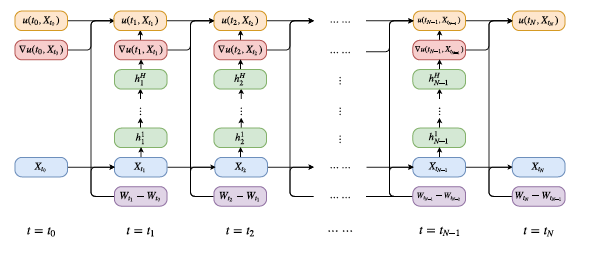
\includegraphics[width=1.0\linewidth, height=4cm]{graphics/arch.png}
\end{figure}
\end{block}
\end{frame}




\begin{frame}
\frametitle{Machine Learning (3)}
\begin{block}{Data}
We sample M price paths  ie.$i=1,\cdots,M$ by \eqref{eq:11}. So we have $X_{t_n}^i$,where $i=1,\cdots,M$  and $t_n=t_0,\cdots,t_N$.\\
The loss function is 
\emph{\alert{$l(\theta,\beta)=\frac{1}{M}\sum_{i=1}^{i=M}(u(t_N,X_{t_N}^i)-C(X_T^i))^2$.}}
We use standard stochastic gradient descent method to find the optimal $\theta^\star$ and $\beta^\star$.
\end{block}
\begin{block}{Experiment }
We sample M=1000 paths and use batchsize$=64$ for  stochastic gradient decent .\\
We set parameters $r=0.04$,$\sigma=0.15$, maturity $T=30$ days and $\xi=100$, strike price $K=100$.\\
With standard BS equation, we know the price of call option is 1.8918,put option is 1.5604 .
%
We use 29 neural networks to approximate $X_{t_n}\frac{\partial u}{\partial x}(t_n,X_{t_n})$ 
for day$s=1,\cdots,29$.
\end{block}
\end{frame}


\begin{frame}
\frametitle{Machine Learning (4)}
\begin{block}{Experiment}
\begin{figure}
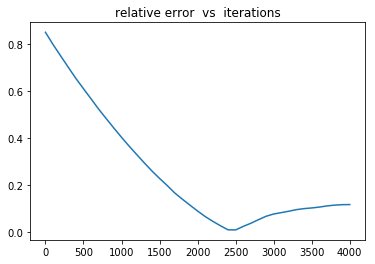
\includegraphics[width=0.6\linewidth, height=2.5cm]{graphics/fig1.png} 
\caption{Call option: price$=1.8918$, $S_0=100$, $K=100$}
\label{fig:subim1}
\end{figure}
%
\end{block}
\end{frame}



\section{Discussion}
\begin{frame}
\frametitle{Discussion(1)}
\begin{itemize}
    \item  Computational complexity does not grow with dimensionality
\end{itemize}
\begin{itemize}
    \item  Relative error goes up after more iterations
\begin{figure}
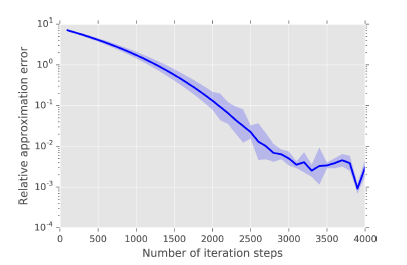
\includegraphics[width=0.6\linewidth, height=2.5cm]{graphics/fig3.png}
\label{fig:subim2}
\end{figure}
\end{itemize}

\begin{itemize}
    \item  Machine learning for other type of PDEs
\end{itemize}
\begin{itemize}
    \item Code :https://bitbucket.org/yiliueth/machine-learning-in-finance
\end{itemize}
\end{frame}


\begin{frame}
\frametitle{Discussion(2)}

\begin{itemize}
    \item  Machine learning for other type PDEs


For example ,consider equation of porous media on the unit square:
\begin{equation*}
    -\nabla \cdot(\sigma \nabla u)=f ,\text{ in }\Omega :(0,1)^2, u=0 ,
    \text{ on } \partial \Omega
\end{equation*}
take 
\begin{align*}
f(x,y) 
&= 4\pi^2 sin(2\pi x) sin(2\pi y)(4 cos(2\pi x) cos(2\pi y) + \pi), \sigma(x,y) \\
&= \frac{\pi}{2} + cos(2\pi x) cos(2\pi y)
\end{align*}
\end{itemize}
\end{frame}


\begin{frame}
\frametitle{Discussion (3)}
\begin{block}{Experiment}
\begin{columns}
\begin{column}[b]{0.49\textwidth}
\begin{center}
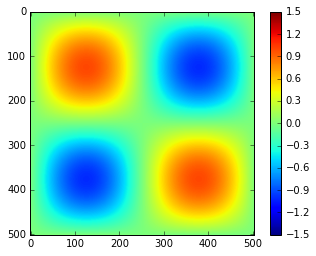
\includegraphics[width=0.8\textwidth]{graphics/FD.png} 
\newline
\inStructColor{Numerical solution} 
\phantom{using boundary conditions and random sparse solution}
\phantom{using boundary conditions and random sparse solution}
\end{center}
\end{column}
\begin{column}[b]{0.49\textwidth}
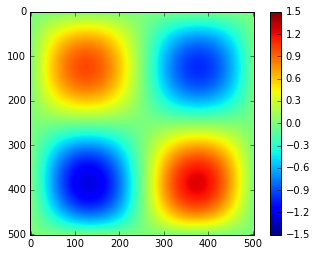
\includegraphics[width=0.8\textwidth]{graphics/GP.png}
\newline
\inStructColor{Machine learning solution, using boundary conditions and random sparse solution}
\end{column}
\end{columns}
\end{block}
\end{frame}

%%%
\begin{appendix}
\begin{frame}<handout:0>[c,plain]
%%\frametitle{The ultimately final remark}
%\addtocounter{framenumber}{-1}
\begin{center}
{\huge\inStructColor{Thank you!}}
\end{center}
\end{frame}
%%%
%
 %
%\begin{frame}
%\frametitle{References}
%\begin{thebibliography}{van der Vaart and Wellner, 1996}
%\bibitem[Mainik and R\"uschendorf, 2010a]{Mainik/Rueschendorf:2010}
%G.\ Mainik and L.\ R\"uschendorf
%\newblock{On optimal portfolio diversification with respect to extreme risks}
%\newblock{Finance and Stochastics, 2010}
%
%\bibitem[Mainik, 2010]{Mainik:2010}
%G.\ Mainik
%\newblock{On Asymptotic Diversification Effects for Heavy-Tailed Risks}
%\newblock{Doctoral thesis, University of Freiburg, 2010}
%
%\bibitem[Mainik and R\"uschendorf, 2010b]{Mainik/Rueschendorf:2010}
%G.\ Mainik and L.\ R\"uschendorf
%\newblock{Ordering of multivariate probability distributions with respect to extreme portfolio losses}
%\newblock{Submitted}
%
% \bibitem[Hauksson et al., 2000]{Hauksson/Dacorogna/Domenig/Mueller/Samorodnitsky:2000}{Hauksson/Dacorogna/Domenig/Mueller/Samorodnitsky:2000}
% Hauksson, Hoskuldur A., Dacorogna, Michel M., Domenig, Thomas, M\"uller, Ulrich  A. and Samorodnitsky, Gennady
% \newblock{{Multivariate Extremes, Aggregation and Risk Estimation}}
% \newblock{available at \texttt{http://ssrn.com/paper=254392}}
%
% \bibitem[Schmidt and Stadtm{\"u}ller, 2006]{Schmidt/Stadtmueller:2006}
% Schmidt, Rafael and Stadtm{\"u}ller, Ulrich,
% \newblock{Non-parametric estimation of tail dependence}
% \newblock{Scand. J. Statist., 2006}
% %
% \bibitem[Balkema and Embrechts, 2004]{Balkema/Embrechts:2004}
% Balkema, Guus and Embrechts, Paul
% \newblock{Multivariate excess distributions}
% \newblock{available at
% \texttt{http://www.math.ethz.ch/~baltes/ftp/guuspe08Jun04.pdf}}
%
% \beamertemplatebookbibitems
% \bibitem[de Haan and Ferreira, 2006]{de_Haan/Ferreira:2006}
% L.\ de Haan and A.\ Ferreira
% \newblock{Extreme Value Theory}
% \newblock{Springer, 2006}
% %
% \bibitem[van der Vaart and Wellner, 1996]{van_der_Vaart/Wellner:1996}
% A.\ W.\ van der Vaart and J.\ A.\ Wellner
% \newblock{Weak Convergence and Empirical Processes}
% \newblock{Springer, 1996}
% %
% \bibitem[M\"uller and Stoyan, 2002]{Mueller/Stoyan:2002}
% A. M\"uller and D.\ Stoyan
% \newblock{Comparison Methods for Stochastic Models and Risks}
% \newblock{Wiley, 2002}
%
%
% \bibitem[Falk et al., 1994]{Falk/Huesler/Reiss:1994}
% Falk, Michael, H{\"u}sler, J{\"u}rg and Reiss, Rolf-Dieter
% \newblock{Laws of small numbers: extremes and rare events}
% \newblock{Birkh\"auser, 1994}
% %
%\end{thebibliography}
%\end{frame}
\end{appendix}
\end{document}
